\subsection{The SVM}
\subsubsection{Preliminary decisions \& notes} \label{svmdecisions}
As described in chapter \ref{The Architecture}, we began our project with the idea of using C\# for every part of the program. When we stumbled into the problems described in aforementioned chapter, we switched to using Python. Specifically, we chose to use the scikit-learn library (hereafter sklearn). This library includes a vast array of classifiers of ways to preprocess data for said classifiers. For the data preprocessing, we went with sklearns TfidfVectorizer\cite{tfidf}.

A problem with using a SVM is that it’s inherently meant for binary problems (eg. is it true or false, is it a car or not etc.).
Since we have five classes if we utilize our fine-grained annotations, or at the minimum three classes if we remap two's and minus two's to one's and minus one's, it’s still one class too many for it to be a binary problem.
An important method to mention before that is that you can handle this as a one-versus-rest problem, meaning that you train a classifier to see if a given input belongs to a specific class or not.
Sklearns SVM implementation handles this by training n\_classes one-versus-rest classifiers, meaning that it will eg. end up with a positive-or-not, neutral-or-not and negative-or-not classifier, and predict over them until it finds the correct class.
An issue with this is that we have no transparency. Two classifiers could claim a phrase belongs to them, ie. one claims positive and another negative, and we have do not know how it handles such issues. We will come back to this problem later.

\subsubsection{Data preprocessing}
For shrinking our classes from 5 different to simply negative, neutral and positive, we check if the number is either 0, negative or positive. If it’s either of the two latter, we just label them -1 or 1 respectively.
The reasoning behind this is that we don’t have enough data to train a classifier with both positive (1) and very positive (2) classes. By going from fine grained labels (5 different classes) to only 3 classes, we improve our accuracy by an average of 15\%. It is important to note that using 5 is only worse in the sense that our classifier has a harder time distinguishing the 5 classes from one another, when looking at the polarity of the predictions - if they were positive, negative or neutral - it remains the same as when squishing the classes.

As a very first step, we lowercase all letters in our sentences. Without this, the same word would be seen as a different word depending on how uppercase or lowercase letters are used.
One could argue that a full capital version of certain words could hold a different sentiment than one without, but it would also see words in the start of sentences as different words, just because their first letter is in uppercase. This would greatly increase the number of words we have not yet seen before and therefore increase the difficulty of classifying them.

At this point in the processing, we attempted stemming the words. Stemming is removing the suffix from a word, leaving you with only the root. It would take words like “haltede” and remove the suffix, leaving us with “halte”. The issue with this is that some words change drastically depending on what tense it is in. The word “spurgte” cannot be converted to “spørge”, just by removing the suffix.
Stemming words could potentially remove the problem of not having seen a specific tense of a word. If our vocabulary includes “love”, but not “loved”, predicting on a sentence that uses “loved” could give wrong results. But if it is stemmed, then it would simply remove the suffix “d”, and end up with “love" which it has already seen.
However, with our dataset, it didn't do a measurable difference. This could come down to our vocabulary being very large, the different tenses of the word not looking alike or spelling errors (of which there are many).

We have made a list of stop words, which are essentially words without any significant sentiment that we remove from the sentences. It can also be words that are used very frequently. Example of such words are: “er”, “du” and “at”, which also coincides within our top 10 most frequent words as seen in \ref{sprogetdk} . The idea is that none of them carry any information that we need, and therefore are not important to us. Yet if we do not remove them, when it has been converted to a vector, it would have to end up with a representation of either positive, negative or neutral, which could distort our results.

After having applied this cleaning to every single sentence, the result is then converted into a sparse matrix representation of the token counts. This means that the number of a said token is increased by one every time it is seen.
We also take a look at n-grams, so that our classifier may better understand words in context to one another. This means that the sentence “Hej med dig”, if we have an n-gram range of 1 to 2, would be split into the following tokens “hej”, “med”, “dig” but also “hej med” and “med dig”.
That way, it can distinguish how words are used in certain contexts, and how their sentiment may change depending upon that.
What we found to be the perfect range for our dataset is 1-3, meaning that it creates unigrams, bigrams and trigrams. Anything less is not enough to convey the context, and anything more decreased our performance while also taking longer to train.

Something different we found to give good results is to tokenize letters instead of words, and use a much larger n-gram range. So instead of looking at a word in context to its surrounding words, we look at letters in context to its surrounding letters within a word. What we end up with is tokens of individual letters, and tokens of letters of length 1 to n. We chose to only look at single words, meaning that if we try to make a trigram of the word “og”, it will only generate the tokens “o”, “g”, and “og”.

The difference between these two are that tokenizing by words will give the classifier a better understanding of which words are used in context to the words around it, whereas tokenizing by characters in a word might help with spelling mistakes.

What then happens is that it the sparse matrix is transformed to a normalized tf or tf-idf representation.
As the documentation for sklearns TfidfTransformer states:
\textit{“The goal of using tf-idf instead of the raw frequencies of occurrence of a token in a given document is to scale down the impact of tokens that occur very frequently in a given corpus and that are hence empirically less informative than features that occur in a small fraction of the training corpus.”} \cite{tfidf} \\
The TFIDF formula is as given:
\begin{itemize}
    \item \textbf{TF}: Term frequency, measures how frequently a term occurs in a document. Since documents differ in length, it is possible a term would appear more often in longer documents than shorter ones. Therefore the term frequency is often divided by the document length as a sort of normalization
    \textit{TF(t) = (Number of times a term appears) / (Total number of terms in document)}
    \item \textbf{IDF}: Inverse Document Frequency, it measures how important a term is. Without this, all terms are seen as equally important. However, certain terms, such as the ones in our list of stop words, are of little importance but may appear often - with that in mind we need to weigh down frequent terms, but scale up the rarer ones.
    \textit{IDF(t) = log e(Total number of documents / number of documents with term t in it)}
\end{itemize}

\begin{itemize}
    \item Use idf: We can choose not to use the inverse document frequency
    \item Smooth idf: Add one to every document frequency. This means that it appears as if an extra document was seen containing every term in the collection exactly once. According to sklearn documentation, it prevents zero divisions.
    \item Sublinear tf: Instead of using the normal tf, replace it with 1 + log(tf) for sublinear scaling.
\end{itemize}
Choosing which of these parameters to use will be discussed further on. What we end up with after this is our data in a higher dimensional space.

For the classifier itself, we started with sklearns SVC\cite{svc} (C-Support Vector Classification), and the first thing we needed to ask ourselves was which kernel to use. To figure this out, we tried with a bunch of different kernels, namely the radial basis function (RBF\cite{rbf}) kernel, a polynomial kernel\cite{poly}, and a linear kernel\cite{linear}. Which one to use will heavily depend on how our data is represented in its high dimensional space. 
After having tried out these different kernels, we found that the linear kernel gave us the best results, with a 10-15\% accuracy increase over the other two. To speed up training, we then switched to sklearns LinearSVC, which is built with a linear kernel in mind.

To better choose which to use, we used sklearns form of hyperparameter tuning: GridSearchCV. It takes a list of whatever parameters relevant to the classifiers and transformers (As our TfidfTransformer) that we want to try out, and it tries out every single possible combination of them, while cross validating with the stratified k-fold method. This lets us tailor the parameters to our data at the expense of training time, while also letting our classifier see all the data in the set.

\begin{figure}[H]
    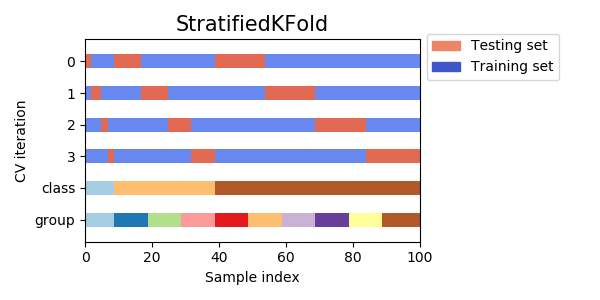
\includegraphics[width=8cm]{Images/StratifiedKFoldExplanation}
    \centering
    \caption{Image showcasing Stratified K-Fold.\cite{stratifiedkfold}}
    \label{StratifiedKfold}
\end{figure}

The k-fold cross validation is a way to split the data into test and training parts. It splits the data into k samples, and then uses one fold for testing while using the rest for training. It does this until every fold has been used for testing, meaning that the classifier will have seen all the data at the end of the cross validation.
Stratified sampling essentially means that each fold will have an equal percentage of the different classes, as can be seen in figure \ref{StratifiedKfold}. Each testing set from each iteration contains the same proportional amount of each class as the rest. For our data, since we have a disproportion of neutral and negative to positive, it ensures that each fold contains positive sentences. Essentially, we can see how our classifier performs on each class, instead of having the possibility of having all the positives in the training set, and none in the test set.

\subsubsection{Custom multiclass SVM}
As described in chapter \ref{svmdecisions}, there is a lack of transparency on the internal picking of a prediction when using our standard SVM. We do not know how it acts on conflicting predictions between the different classifiers on the same phrase. That was the motivation for us to create a script where we have full control over these decisions. The core idea behind it is that we have two classifiers: one checks if it is negative or not, and the other checks if it is positive or not. If it is neither positive nor negative, then it’s neutral. The data preprocessing will be the same as for the ordinary SVM, with the only difference being how the data is labelled.

The negative-or-rest classifier is trained on the same dataset as the positive-or-not classifier, but the labels are altered for the two. For the former, the labels are either -1 for negative, 0 for non-negative. For the latter, it’s 1 for positive, 0 for non-positive. This means that for the former, both positive and neutral are labelled with a 1.
The reason for this is the following:
When predicting, both classifiers will return their prediction - either -1 or 0 for the negative-or-rest, or 1 and 0 for the positive-or-rest -  which will be added together.
If the result of adding these two together is -1 (negative-or-rest predicted -1, positive-or-rest predicted 0, -1 + 0 equalling -1), then it’s negative, and vice-versa if the result is 1.
Here is a full list of the results and what they mean:
\begin{itemize}
    \item -1: Negative-or-rest has predicted negative, positive-or-rest has predicted non-positive. This means that it predicts negative.
    \item 1: Negative-or-rest has predicted non-negative, positive-or-rest has predicted positive. This means that it predicts positive.
    \item 0: This can mean one of two things: either both claimed the phrase does not belong to their primary category, and thus have both returned 0 (0 + 0 = 0), OR it means that both claim it belongs to their respective primary class (-1 + 1 = 0). In this case, we simply claim that it’s neutral.
\end{itemize}
So with simple arithmetic, we have created the transparency and control that we wish to have over the classifiers. What more is that we have done it with one classifier less than standard sklearn LinearSVC (recall that it trains the same amount of classifiers as there are classes).

\subsubsection{Kernel choice}
The very first thing we wished to figure out is how our data would look like as a 2D representation. The thought behind this was that we would be better suited to figure out which kernel to use if we could observe how our data behaves when it has been transformed into a higher dimension space. To this end, we used t-distributed stochastic neighbour embedding (TSNE\cite{tsne}) to get a better look. As for the parameters, we used the default ones, except decompose\_by, which we set to 25.
\begin{figure}[H]
    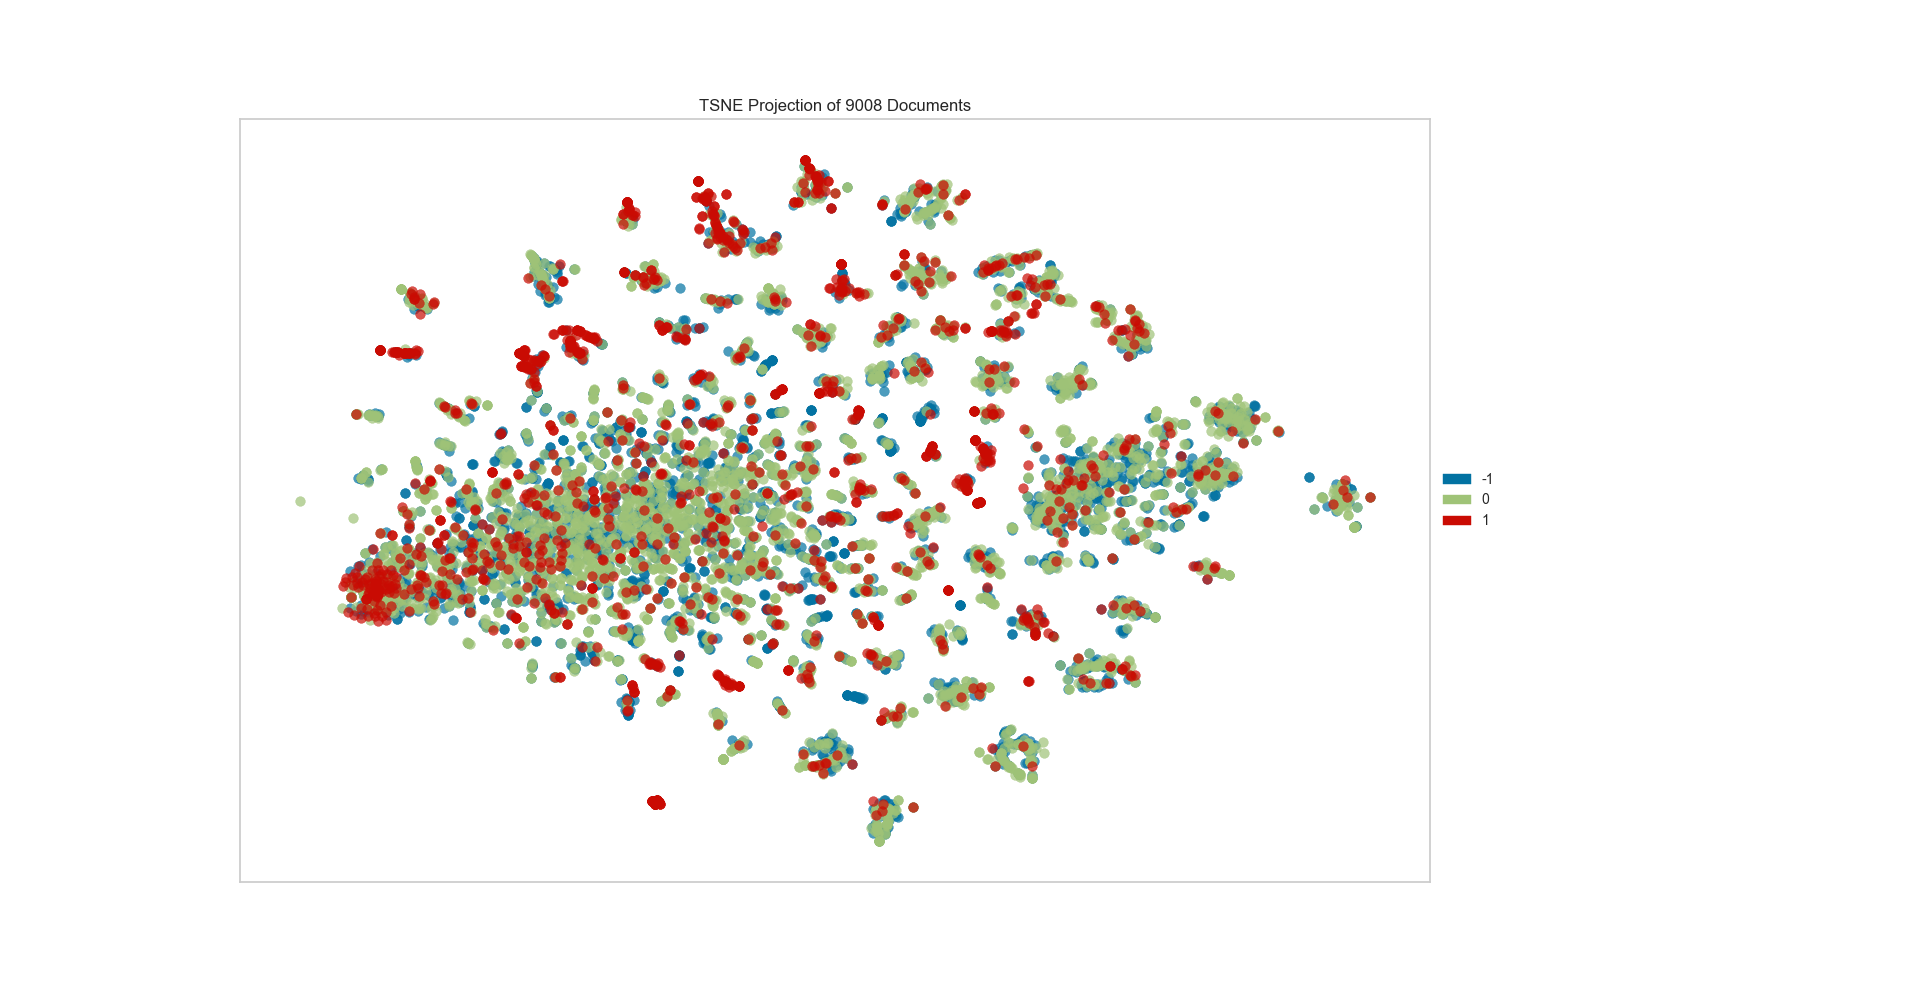
\includegraphics[width=14cm]{Images/TSNEProjectionWord}
    \centering
    \label{TSNEProjectionWord}
\end{figure}
What this graph shows is a projection of our data when using a word tokenizer with an n-gram range of 1-3. The number of dimensions this data exists in normally is 78000, which is the number of features we have in this case.
As can be seen from this graph, the data overlaps a lot. This could either mean that our problem is non-linear, meaning that we cannot seperate the different classes with a linear kernel. It could also be that the way we perform dimensionality reduction doesn't properly represent the data when it has been reduced to a 2D representation.
While it doesn't look like the problem is linearly seperable, we tried out different kernels to see which ones work the best. We tested a radial basis function (RBF) kernel, a linear kernel and a polynomial kernel. What then comes as a surprise is that a linear kernel outperforms every other kernel.
Here are the results of the different kernels
\begin{itemize}
    \item Linear kernel: ~65\% accuracy
    \item RBF kernel: ~45\% accuracy
    \item Polynomial kernel: ~40\% accuracy
\end{itemize}
From these results, we decided to go with a linear kernel and sklearns linear SVM implementation (as described earlier)¸ which has the added bonus of a quicker training time.

\subsubsection{Classifier confusion}
After having trained our classifier, we decided to create a confusion matrix to test our classifiers accuracy and performance over the different classes. 
\begin{figure}[H]
	\centering
	\subfloat[Image of the confusion matrix.]{
		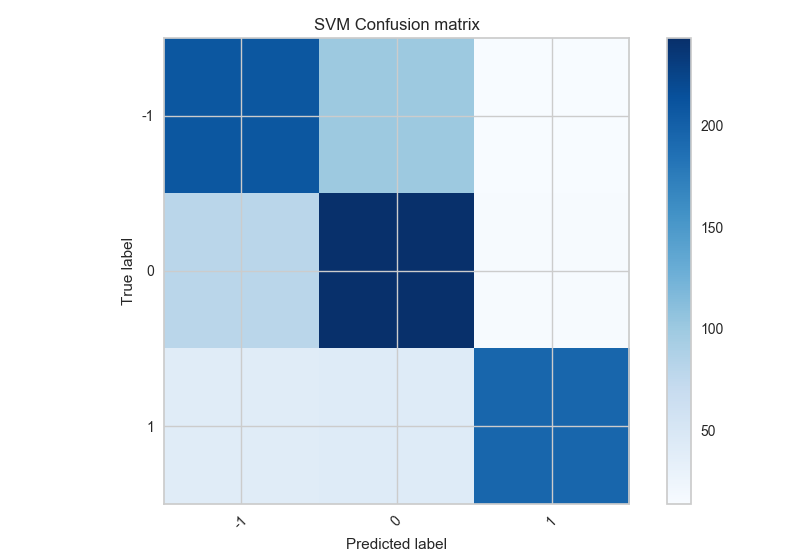
\includegraphics[width=0.5\textwidth]{Images/ConfusionMatrixThreeClassesSVM}
		\centering
		\label{ConfusionMatrix}	
	}
	\subfloat[Table of the confusion matrix.]{			
		\begin{tabular}{@{}llllll@{}}
			\toprule
			& & \multicolumn{3}{c}{Predicted} \\\cmidrule{3-5}
			Actual & & Negative & Neutral & Positive &  \\ \midrule
			Negative & & 209 & 100 & 14 & \\
			Neutral  & & 80  & 243 & 15 & \\
			Positive & & 40  & 42 & 195 & \\ \bottomrule
		\end{tabular}
		\centering
		\label{tableofconfusion}
	}
\end{figure}
The primary issue with our classifier is that it has trouble distinguishing between neutral and negative sentences.

\subsubsection{Tokenizing words or characters}
As described earlier, we can either tokenize the given phrases on a word-by-word basis or on a character-by-character basis. To test this we've run both methods 100 times and written down the results. The results from word tokenizing can be seen on table \ref{wordtokenresult}. 
\begin{table}[H]
	\begin{tabular}{@{}lll@{}}
		\toprule
		Accuracy & word    &         \\ \midrule
		Minimum & Average & Maximum \\
		56.38\%  & 60.63\% & 64.15\% \\ \bottomrule
	\end{tabular}
	\centering
	\caption{Results with word tokenizing}
	\label{wordtokenresult}
\end{table}

When utilizing character tokenisation, we get the results as seen on table \ref{chartokenresult}.

\begin{table}[H]
	\begin{tabular}{@{}lll@{}}
		\toprule
		Accuracy & char\_wb &         \\ \midrule
		Minimum  & Average  & Maximum \\
		60.49\%  & 66.12\%  & 69.03\% \\ \bottomrule
	\end{tabular}
	\centering
	\caption{Results using character tokenisation.}
	\label{chartokenresult}
\end{table}

Tokenizing with characters gives us an average increase of 6\% points over tokenizing with words.

\subsubsection{Names and topics}
An observation we made during testing is that after training, names and topics that were discussed in one topic could skew the prediction of testing sets that contain the same names and topics. As an example, the classifier thinks that "Pia Kjærsgaard" is positive, and the name has such a force behind it that almost every sentence with that name in it that we tested with would be classified as positive, even though they contained some rather nasty words. So if we wanted to predict the sentiment of a phrase where the subject is Pia Kjærsgaard, like the sentence "Pia Kjærsgaard er forfærdelig", even though the sentiment of the phrase towards her is negative, her name has been used primarily in a positive context, and it would predict wrongly. Other names and topics could be Esben Lunde Larsen or vaccines.

By updating our list of stop words to contain topics and names, the lower bound of our confidence interval increased from 60,5\% to 62,62\% as can be seen on table \ref{stopwords}. That is, our lowest score increased by 2\%. At the same time, our highest score increased by almost 1\%. The average score decreased slightly. 
\begin{table}[H]
	\begin{tabular}{@{}lll@{}}
		\toprule
		Accuracy & char\_wb &         \\ \midrule
		Minimum  & Average  & Maximum \\
		62.62\%  & 66\%  & 69.9\% \\ \bottomrule
	\end{tabular}
	\centering
	\caption{Results with updated stop words.}
	\label{stopwords}
\end{table}

The better confidence interval and average accuracy is only one of the reasons we've chosen to go with tokenizing characters instead of words. Another reason is that we believe it handles light spelling mistakes better than word tokenizing. Where word tokenizing only takes into account the words already seen, character tokenizing will be able to correct slight spelling mistakes on some words by comparing parts of the word to something it has already seen.
As an example, both methods of tokenizing will result in the classifiers to correctly predict the phrase \textit{forfærdeligt træls} as being negative. If we feed both of them with the misspelled phrase \textit{forfærdligt træl}, the classifier with a word tokenizer wrongly predicts it to be neutral, whereas the character tokenizer correctly predicts it to be negative. Our assumption is that since the character tokenizer has already seen tokens such as \textit{forfærd} from \textit{forfærdeligt}, the tokens help the classifier understand the relation of the tokens to the words they originate from.

\subsubsection{Custom multiclass SVM accuracy}
When trying out our own multiclass SVM built using sklearns library, we achieve results that resembles the ones before very much. This one uses both the updated stop words and a character tokenizer. The differences lie in an average and maximum that both are slightly lower by 0,41\% and 0,31\% respectively, but a minimum that is higher by 1,31\%. 
\begin{table}[H]
	\begin{tabular}{@{}lll@{}}
		\toprule
		Accuracy & char\_wb &         \\ \midrule
		Minimum  & Average  & Maximum \\
		63.93\%  & 65.59\%  & 69.59\% \\ \bottomrule
	\end{tabular}
	\centering
	\caption{Results with updated stop words.}
	\label{stopwords}
\end{table}
What we've discovered by looking at the accuracy results of the cross validations from the two different classifiers that constitute this multiclass SVM (negative-or-rest \& positive-or-rest), we see a general pattern.
\begin{itemize}
	\item The positive-or-rest classifier generally scores between 87-88\% accuracy.
	\item The negative-or-rest classifier generally scores between 64-68\% accuracy.
\end{itemize}
As can be seen, differentiating between positives and non-positives is easy with our dataset, whereas it is slightly harder differentiating between negatives and non-negatives.

\subsection{Refresher}
In this section we described how we preprocess the data before we vectorize it. We described the different approaches we had to the SVM and why we use the linear kernel with n-grams of 1-10 with characters and word bounds.
